%# -*- coding: utf-8-unix -*-
%%==================================================
%% chapter01.tex for SJTU Master Thesis
%%==================================================

%\bibliographystyle{sjtu2}%[此处用于每章都生产参考文献]
\chapter{qscache系统测试}
\label{chap:sys_test}

qscache系统的测试工作由测试目标与测试方法、qscache系统性能测试、qscache系统功能性测试这三个部分组成,接下来将分别进行介绍。

\section{测试目标与测试方法}

\subsection{测试目标}

测试目标为检验对于qscache系统的设计是否都有达到预期,即qscache系统是否具有大容量、低成本、高顺序读写性能、高随机读写性能并且支持多缓存设备对多后台设备、I/O带宽按权限分配。

qscache系统中,缓存设备与后台设备作为Device Mapper的target device被加载到系统中,qscache系统的容量取决于被加载的后台设备的容量。只要系统能支持多缓存设备、多后台设备,那么qscache系统就能以多块HDD作为后台设备提供大存储容量。在qscache系统中,缓存设备的容量一般取后台设备的十分之一到八分之一,对于1TB的HDD作为后台设备,取128G的SSD作为缓存设备,系统的成本还是可接受的。因此,测试的内容主要落在qscache系统的性能上以及qscache系统是否支持I/O带宽按权限分配,需要对qscache系统的顺序读写性能与随机读写性能进行测试,验证是否达到预计目标。另外需要开启多个进程设置不同权限,验证不同进程被分配到的I/O带宽是否按权限分配。

\subsection{测试方法}

综合qscache的测试目标,本研究对qscache的性能测试主要采用对比的方法,对比的系统包括:基于HDD的存储系统、开源混合存储系统flashcache、本系统qscache。对于qscache是否支持I/O带宽按权限分配,本研究采用普通的测试方法,通过开启多个测试进程,为不同测试进程设置不同权限,查看不同测试进程最后给出的性能统计进行验证。

\section{测试环境}

测试环境如表\ref{tab:qscache_test_environment}所示

\begin{table}[H]
    \zihao{5}
    \centering
    \bicaption[tab:qscache_test_environment]{qscache性能测试环境}{qscache性能测试环境}{Table}{test environment of qscache}
    \begin{tabular}{cc} \toprule
      机器类型 & 普通台式机 \\ \midrule
      CPU & 单核AMD CPU\\
      内存 & 1GB DDR3\\
      SSD & 120GB intel350 \\
      HDD & WD 1TB 7200rpm绿盘\\
      内核版本 & 3.10.108\\
      \bottomrule
    \end{tabular}
\end{table}

\section{qscache性能测试}

\subsection{系统初始化}

假设Linux系统中,120GB的SSD为/dev/sdb,1TB的HDD为/dev/sdi。首先对基于HDD的系统进行测试,然后对flashcache系统进行测试,之后对Linux内核进行修改、编译、安装,然后对qscache系统分别采用基于bio的模式与基于request的模式分别进行测试。

对内核修改后,内核的编译安装过程如下:

\begin{enumerate}
    \item cp /boot/config-3.10.0-693.5.2.el7.x86\_64 .config
    \item 在系统原有的内核配置文件的基础上建立新的编译选项:sh -c \lq yes \lq\lq\rq\rq | make oldconfig \rq
    \item 生成内核文件:make bzImage
    \item 编译模块:make modules
    \item 编译安装模块:make modules\_install
    \item 安装:make install
    \item reboot加载新内核
\end{enumerate}

四个系统的初始化操作如下:

\begin{enumerate}
    \item 基于HDD的系统的初始化
          \begin{enumerate}
              \item 无
          \end{enumerate}
    \item flashcache的初始化
    \begin{enumerate}
        \item 编译,需要内核的源码树:make KERNEL\_TREE=/usr/src/linux-3.10.108/
        \item 加载:insmod src/flashcache.ko
        \item 以写回模式创建系统,缓存设备容量120GB,后台设备容量1TB,mapped device命名为cachedev:flashcache\_create -p back cachedev /dev/sdb /dev/sdi
    \end{enumerate}
    \item 基于bio的qscache的初始化
    \begin{enumerate}
        \item 编译,需要内核的源码树:make KERNEL\_TREE=/usr/src/linux-3.10.108/
        \item 加载,以基于bio的模式加载:insmod src/qscache.ko request\_based=0
        \item 以写回模式创建系统,缓存设备容量120GB,后台设备容量1TB,mapped device命名为cachedev:qscache\_create -p back -n cachedev -c /dev/sdb -h /dev/sdi
    \end{enumerate}
    \item 基于request的qscache的初始化
    \begin{enumerate}
        \item 编译,需要内核的源码树:make KERNEL\_TREE=/usr/src/linux-3.10.108/
        \item 加载,以基于request的模式加载:insmod src/qscache.ko request\_based=1
        \item 以写回模式创建系统,缓存设备容量120GB,后台设备容量1TB,mapped device命名为cachedev:qscache\_create -p back -n cachedev -c /dev/sdb -h /dev/sdi
    \end{enumerate}
\end{enumerate}

\subsection{顺序读写性能对比}

顺序读写性能使用fio进行测试,文件大小为4GB,块大小从4KB到16MB,命令为fio -filename=/dev/mapper/cachedev -direct=1 -iodepth1 -thread -rw=RW -ioengine=libaio -bs=BS -size=4G -numjobs=8 -runtime=30 -name=readtest,通过设置BS来设置块大小,通过设置RW为read或write来设置顺序读或顺序写。顺序读写性能测试结果如表\ref{tab:seq_comparison}所示。

\begin{table}[!ht]
    \zihao{5}
    \centering
    \bicaption[tab:seq_comparison]{HDD、flashcache、qscache顺序读写性能}{HDD、flashcache、qscache顺序读写性能(KB/s)}{Table}{ sequential I/O performance contrast among HDD, flashcache and qscache(KB/s)}
    \begin{tabular}{@{}ccccccccc@{}} 
      \toprule
      \multirow{2}*{块大小} & \multicolumn{2}{c}{HDD} & \multicolumn{2}{c}{flashcache} & \multicolumn{2}{c}{bio-qscache} & \multicolumn{2}{c}{request-qscache}\\
      & read & write & read & write & read & write & read & write\\
      \midrule
      4KB & 203686 & 202350 & 184067 & 113235 & 184395 & 110970 & 175886 & 106754\\
      8KB & 211129 & 229899 & 187215 & 135352 & 181659 & 125204 & 173932 & 110897\\
      16KB & 196616 & 203539 & 171163 & 128776 & 172225 & 116473 & 164517 & 114719\\
      32KB & 190884 & 194822 & 159974 & 131076 & 162917 & 115747 & 160245 & 104128\\
      64KB & 184689 & 181444 & 153915 & 141162 & 166891 & 115823 & 164157 & 110325\\
      128KB & 208728 & 214504 & 181982 & 145134 & 164893 & 118921 & 137718 & 106245\\
      256KB & 222185 & 200914 & 189187 & 127656 & 189762 & 105847 & 167462 & 103723\\
      512KB & 229497 & 193496 & 187896 & 105086 & 198944 & 118349 & 156784 & 105581\\
      1MB & 204723 & 211884 & 173823 & 126227 & 164305 & 115985 & 157783 & 102373\\
      2MB & 208785 & 201776 & 187231 & 124686 & 177806 & 115864 & 167256 & 108699\\
      4MB & 261920 & 260618 & 196758 & 125859 & 185505 & 116010 & 165823 & 101882\\
      8MB & 232480 & 220825 & 206443 & 134810 & 199202 & 104759 & 186614 & 94646\\
      16MB & 234581 & 210528 & 201457 & 122041 & 191742 & 113412 & 189106 & 105182\\
      \bottomrule
    \end{tabular}
\end{table}

四者的顺序读性能对比如图\ref{fig:seq_read_comparison}所示,可以看到基于HDD的系统的吞吐量能达到220MB/s,而flashcache大约为170MB/s,基于bio的qscache和flashcache差不多也在170MB/s左右,而基于request的qscache大约为160MB/s。这是因为,对于基于HDD的系统而言,读请求直接在HDD上进行操作,不需要经历额外步骤;而对于flashcache,虽然会设置过滤顺序读写操作不进行缓存,但是对于顺序读写操作的判断比较简单,因此仍有不少被判断为需要被缓存,这些数据块需要先访问SSD查询缓存是否命中,如果未命中还需要去HDD中读取数据并可能会替换缓存,因此额外开销较多;对于基于bio的qscache,由于总体设计和策略与flashcache差不多,因此性能相近;对于基于request的qscache,由于将原本立刻提交的bio请求延缓放入request中,因此性能有所下降。

\begin{figure}[H]
    \centering
    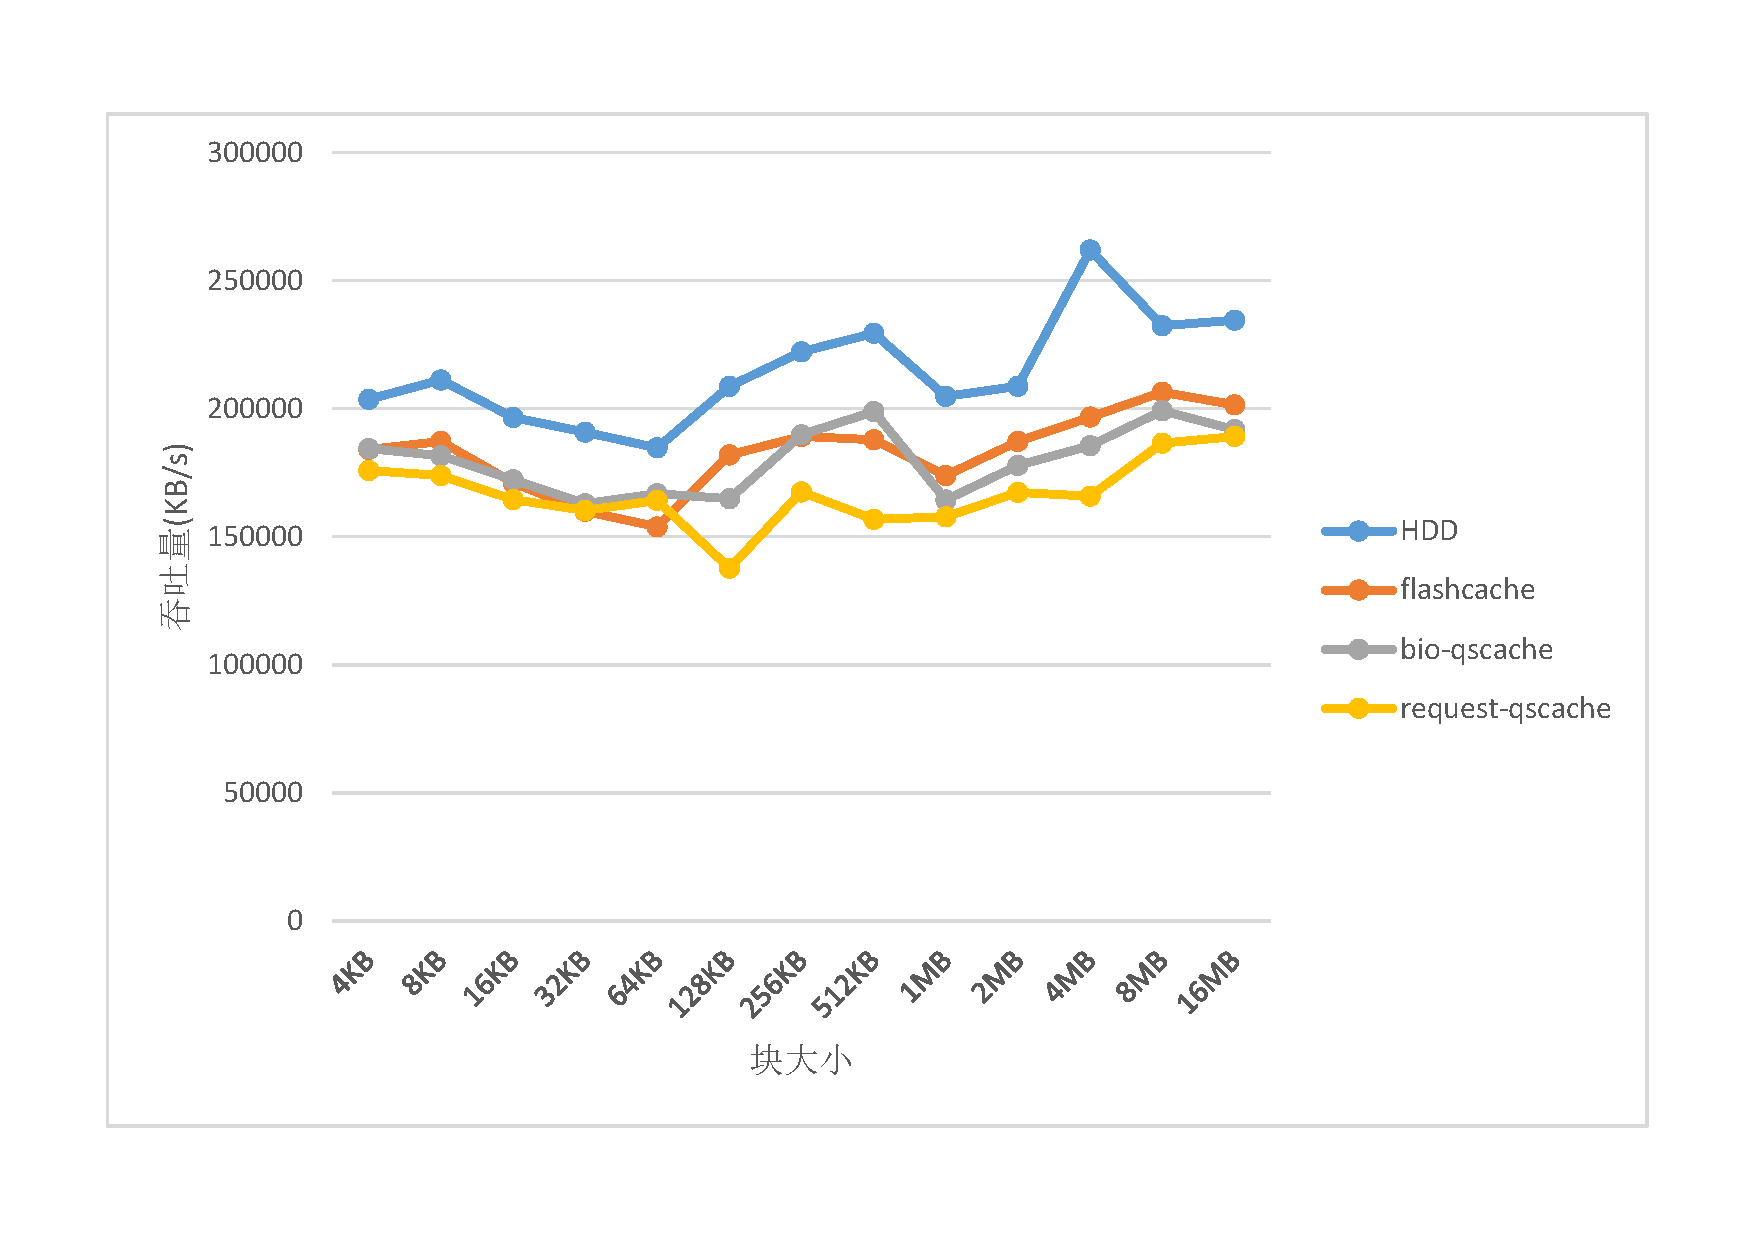
\includegraphics[width=0.8\textwidth]{seq_read.pdf}
    \bicaption[fig:seq_read_comparison]{HDD、flashcache、qscache顺序读性能对比图}{HDD、flashcache、qscache顺序读性能对比图}{Fig.}{ sequential read performance contrast among HDD, flashcache and qscache}
\end{figure}

四者的顺序写性能对比如图\ref{fig:seq_write_comparison}所示,可以看到基于HDD的系统的吞吐量能达到200MB/s,而flashcache大约为130MB/s,基于bio的qscache差不多在110MB/s左右,而基于request的qscache和基于bio差不多,大约为110MB/s。这是因为,对于基于HDD的系统而言,写请求直接向HDD上写数据,不需要经历额外步骤;对于flashcache,与顺序读操作一样,有的数据块仍被判断为需要被换攒,对这些数据块先访问SSD查询缓存是否命中,如果未命中还需要去HDD中读取数据并可能会替换缓存,然后对缓存中的数据进行更改,并会发生写回,因此额外开销较多;对于基于bio的qscache,虽然总体设计和策略与flashcache差不多,但是由于qscache运行在修改过的内核上,因此内核中额外的判断操作使得基于bio的qscache性能不如flashcache;对于基于request的qscache,相比基于bio的qscache除了内核中额外的判断操作外,还需要额外的内核操作以将原本立刻提交的bio请求延缓放入request中,因此性能更加下降。

\begin{figure}[H]
    \centering
    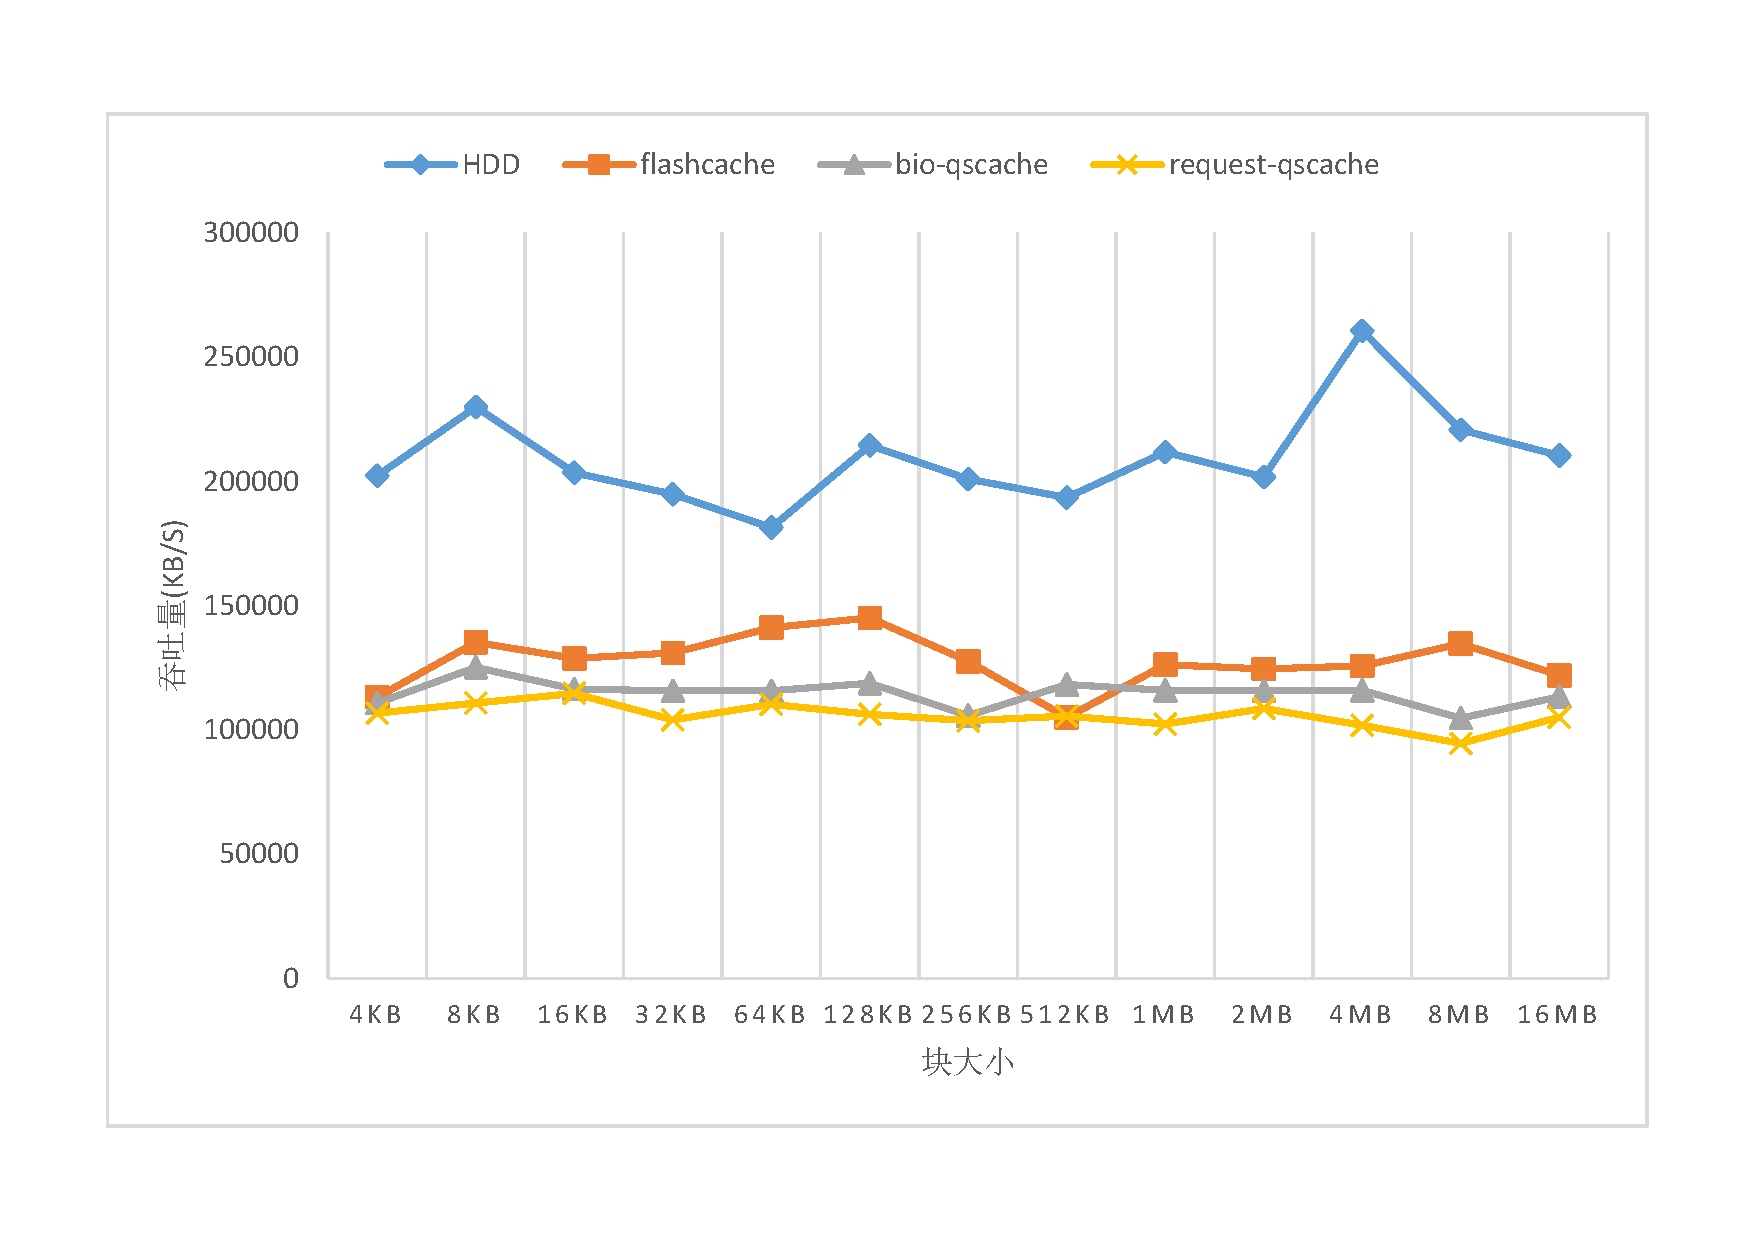
\includegraphics[width=0.8\textwidth]{seq_write.pdf}
    \bicaption[fig:seq_write_comparison]{HDD、flashcache、qscache顺序写性能对比图}{HDD、flashcache、qscache顺序写性能对比图}{Fig.}{sequential write performance contrast among HDD, flashcache and qscache}
\end{figure}

另外可以发现与顺序读操作测试相比,顺序写操作测试中,flashcache和两种模式的qscache系统的性能与基于HDD的系统差距更大。这一方面是由于SSD的写操作相比读操作更费时,因此那些落在SSD上执行的写操作相比读操作会使系统整体性能下降的更明显,另一方面,对于落在SSD上的读操作,不需要考虑缓存容量是否够用,因为缓存中的数据量并不会增加,但是对于落在SSD上的写操作,需要额外考虑缓存的剩余容量,因为可能发生追加数据后需求的总缓存容量大于可用的缓存容量,因此会多层额外的判断,并且可能会相应发生将缓存中其他数据写回的操作。

\subsection{随机读写性能对比}

随机读写性能使用fio进行测试,文件大小为4GB,块大小从4KB到16MB,命令为fio -filename=/dev/mapper/cachedev -direct=1 -iodepth1 -thread -rw=RW -ioengine=libaio -bs=BS -size=4G -numjobs=8 -runtime=30 -name=readtest,通过设置BS来设置块大小,通过设置RW为randread、randwrite或randrw来设置随机读、随机写或混合随机读写。随机读写性能测试结果如表\ref{tab:rand_comparison_1}及表\ref{tab:rand_comparison_2}所示。

\begin{table}[H]
    \zihao{5}
    \centering
    \bicaption[tab:rand_comparison_1]{HDD、flashcache、qscache随机读写性能}{HDD、flashcache、qscache随机读写性能(IOPS)}{Table}{ random I/O performance contrast among HDD, flashcache and qscache(IOPS)}
    \begin{tabular}{@{}ccccccccc@{}} 
      \toprule
      \multirow{2}*{块大小} & \multicolumn{3}{c}{HDD} & \multicolumn{3}{c}{flashcache} \\
      & read & write & read(70\%)/write(30\%) & read & write & read(70\%)/write(30\%)\\
      \midrule
      4KB & 247 & 226 & 143/152 & 21203 & 10843 & 8028/3438\\
      8KB & 213 & 232 & 135/147 & 11277 & 11673 & 6681/2863\\
      16KB & 223 & 227 & 141/144 & 8224 & 10854 & 4727/2030\\
      32KB & 207 & 211 & 135/143 & 4227 & 8949 & 3417/1464\\
      \bottomrule
    \end{tabular}
\end{table}

\begin{table}[H]
    \zihao{5}
    \centering
    \bicaption[tab:rand_comparison_2]{HDD、flashcache、qscache随机读写性能(续)}{HDD、flashcache、qscache随机读写性能(IOPS)(续)}{Table}{ random I/O performance contrast among HDD, flashcache and qscache(IOPS)(continued)}
    \begin{tabular}{@{}ccccccccc@{}} 
      \toprule
      \multirow{2}*{块大小} & \multicolumn{3}{c}{bio-qscache} & \multicolumn{3}{c}{request-qscache}\\
      & read & write & read(70\%)/write(30\%) & read & write & read(70\%)/write(30\%)\\
      \midrule
      4KB & 11812 & 11227 & 7368/3153 & 13649 & 13123 & 8428/3607\\
      8KB & 10286 & 9913 & 6169/2644 & 14251 & 9312 & 6317/2709\\
      16KB & 6284 & 8692 & 4869/2090 & 8929 & 7140 & 4347/1868\\
      32KB & 4650 & 8498 & 3320/1423 & 5785 & 4925 & 2693/1152\\
      \bottomrule
    \end{tabular}
\end{table}


四者的随机读性能对比如图\ref{fig:rand_read_comparison}所示,随机写性能对比如图\ref{fig:rand_write_comparison}所示,可以看到基于HDD的系统在随机读写方面性能,IOPS大约只有200-300,而flashcache和基于bio的qscache以及基于request的qscache的IOPS大约在5000到15000,说明SSD很好地发挥了缓存的作用,使随机读写性能不再是HDD的量级,总的来看flashcache和基于bio的qscache和基于request的qscache在随机读方面性能比较相近,而在随机写方面flashcache和基于bio的qscache性能相近而基于request的qscache性能则较差。

\begin{figure}[!htbp]
    \centering
    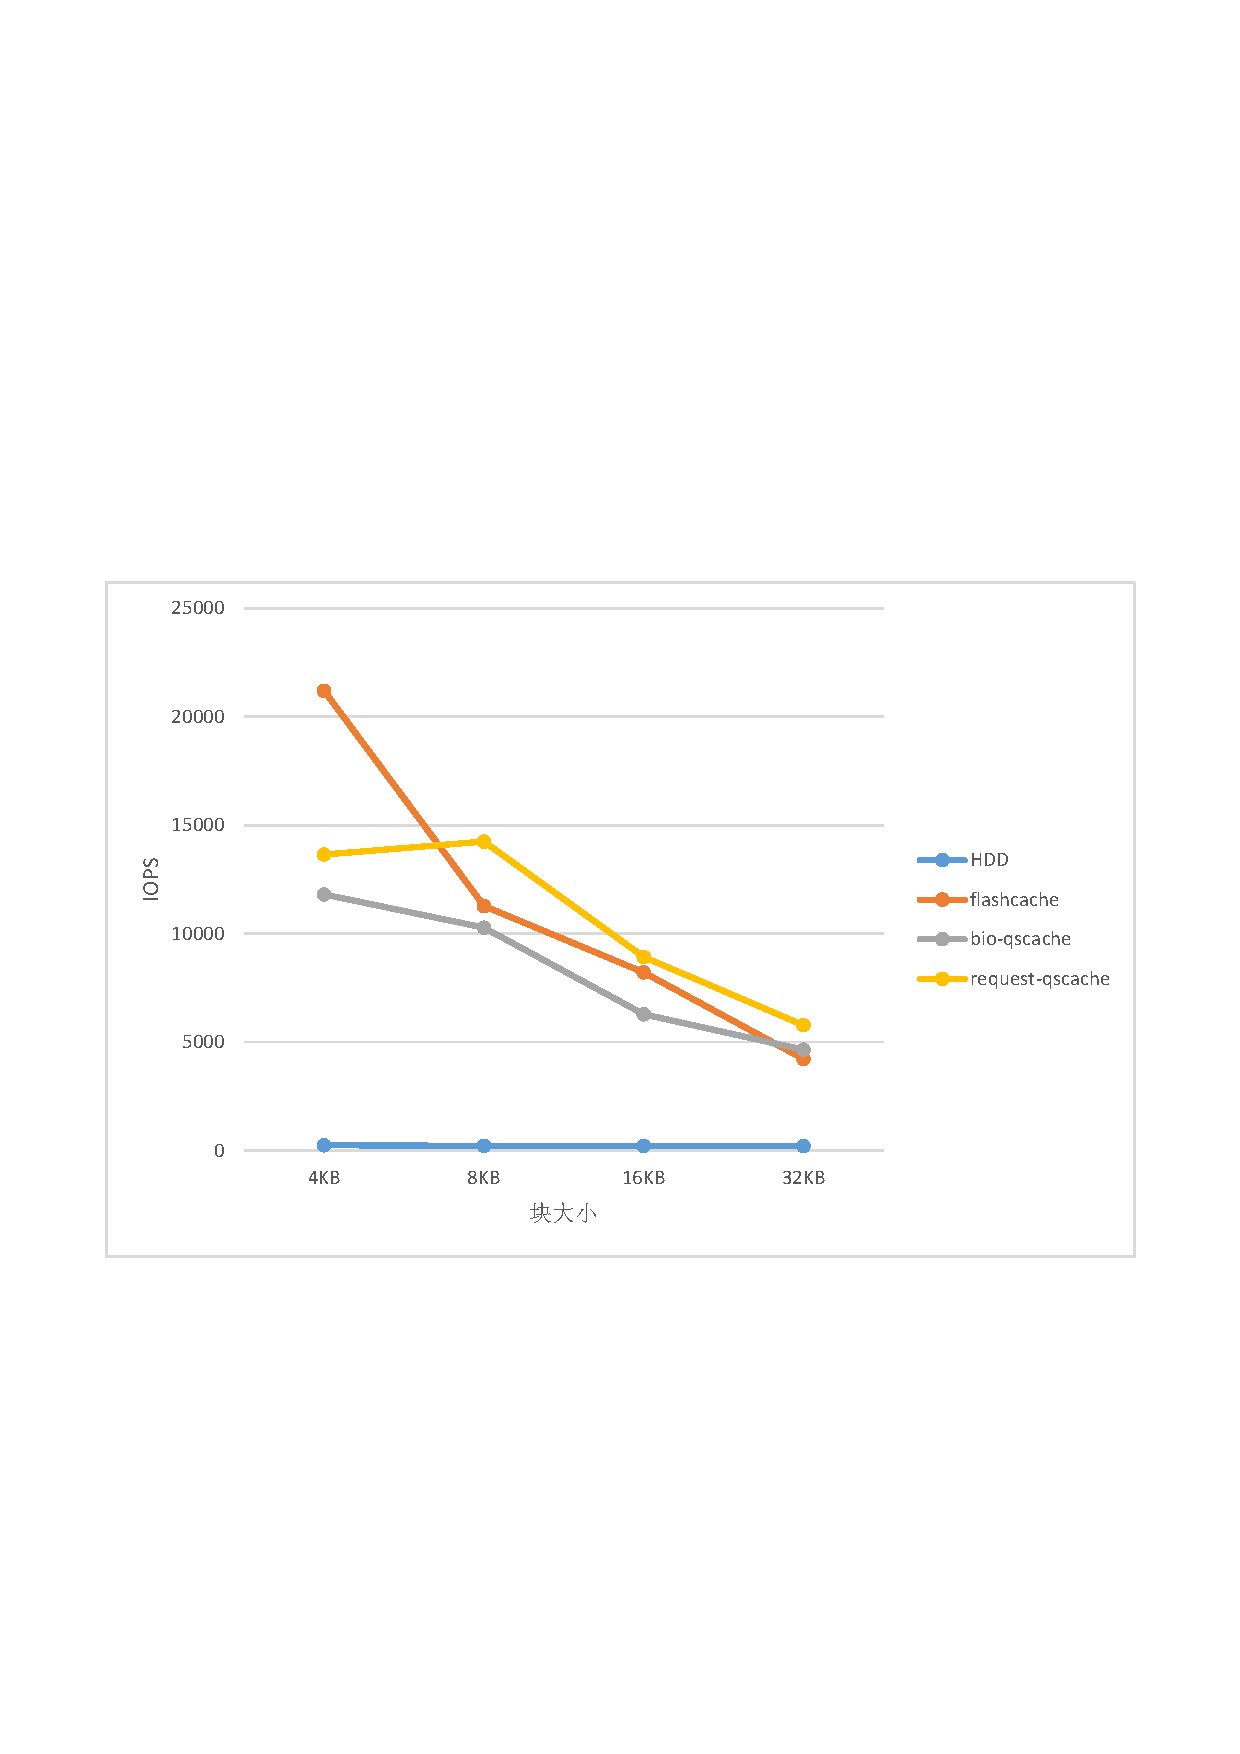
\includegraphics[width=0.8\textwidth]{rand_read.pdf}
    \bicaption[fig:rand_read_comparison]{HDD、flashcache、qscache随机读性能对比图}{HDD、flashcache、qscache随机读性能对比图}{Fig.}{random read performance contrast among HDD, flashcache and qscache}
\end{figure}

\begin{figure}[!htbp]
    \centering
    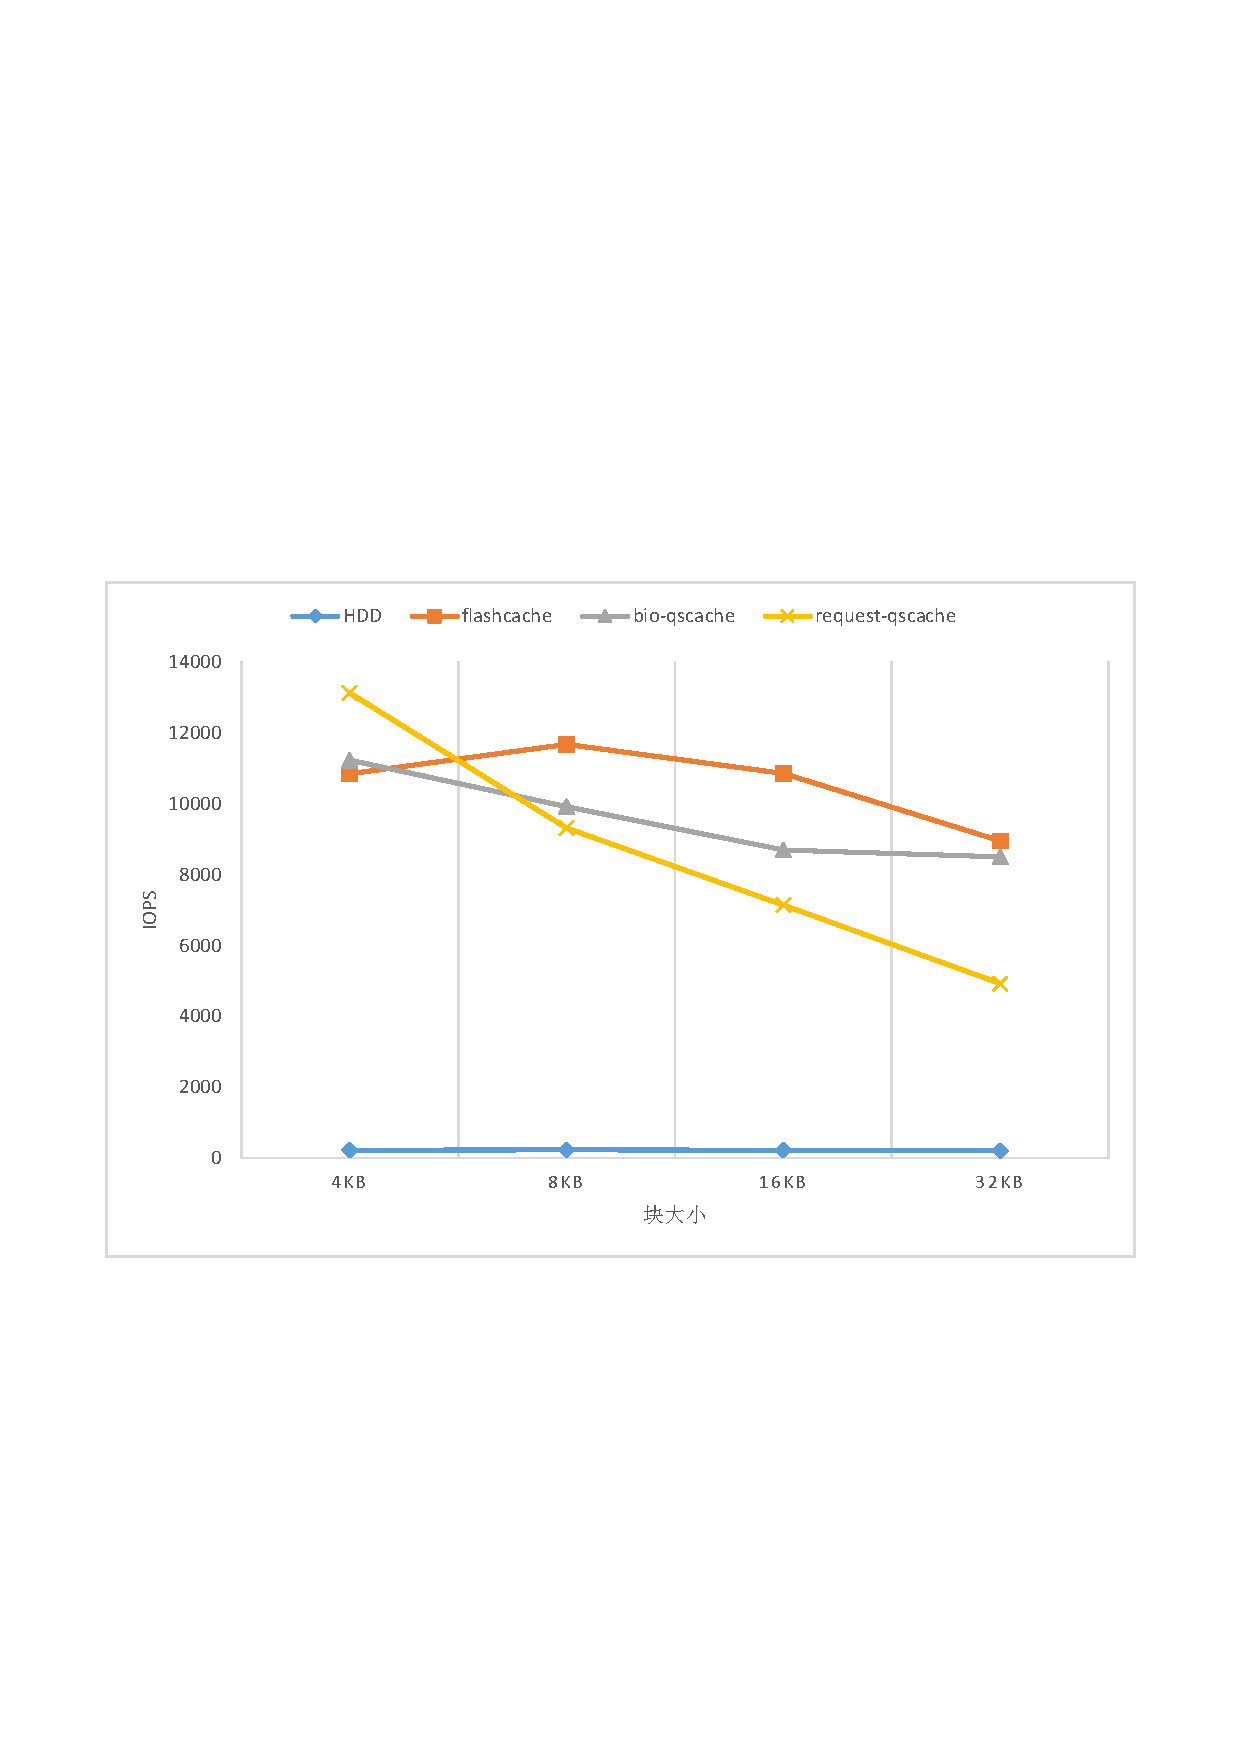
\includegraphics[width=0.8\textwidth]{rand_write.pdf}
    \bicaption[fig:rand_write_comparison]{HDD、flashcache、qscache随机写性能对比图}{HDD、flashcache、qscache随机写性能对比图}{Fig.}{ random write performance contrast among HDD, flashcache and qscache}
\end{figure}

其次可以发现相比顺序读写测试,随机读写测试下flashcache和两种模式的qscache的性能随着I/O的增大性能的波动更大,这是由于当I/O块增大时,每个随机I/O块覆盖的连续数据块更多,因此对越大的I/O块,更有可能被判断为顺序读写的一部分而将操作定性为不需要缓存的操作,从而将这些I/O操作绕过缓存直接在HDD上执行,因此性能产生比较大的波动。

另外注意到基于request的qscache的随机写性能比随机读性能衰减得更厉害,这是由于基于request模式下,request队列的I/O调度默认使用deadline调度策略,在该策略下,会有读I/O的FIFO队列以及写I/O的FIFO队列,读队列最大等待时间为500ms,写队列最大等待时间为5s,之所以会等待是为了在使用HDD时将相邻I/O合并从而提升性能,但是对qscache系统而言,多数请求会落在SSD上执行,但对SSD而言是否合并相邻I/O对性能意义不大。因此相应的写队列更长的等待时间导致写性能更差。

\section{I/O带宽按权限分配测试}

qscache以基于request的模式启动,初始化操作如下:

\begin{enumerate}
    \item 编译,需要内核的源码树:make KERNEL\_TREE=/usr/src/linux-3.10.108/
    \item 加载,以基于request的模式加载:insmod src/qscache.ko request\_based=1
    \item 以写回模式创建混合存储系统,缓存设备容量120GB,后台设备容量1TB,mapped device命名为cachedev:qscache\_create -p back -n cachedev -c /dev/sdb -h /dev/sdi
    \item I/O scheduler使用cfq:echo cfq > /sys/block/dm-2/queue/scheduler
\end{enumerate}

对I/O带宽按权限分配的测试采用fio工具,通过设置fio的不同group的cgroup的weight设置不同测试进程的权限值并测试他们对系统的mapped device的读写性能是否按照权限进行分配。测试结果如表\ref{tab:qscache_io_test}所示,分多组测试,每组测试的cgroup的weight分别设置不同值,可以看到每组测试中I/O带宽按照权重分配了。

\begin{table}[!hpb]
    \zihao{5}
    \centering
    \bicaption[tab:qscache_io_test]{qscache I/O带宽按权限分配测试}{qscache I/O带宽按权限分配测试}{Table}{qscache  I/O quota test}
    \begin{tabular}{@{}cccccccccc@{}} 
        \toprule
        \multicolumn{5}{c}{weight} & \multicolumn{5}{c}{IOPS}\\
        group1 & group2 & group3 & group4 & group5 & group1 & group2 & group3 & group4 & group5 \\
        \midrule
        1000 & 800 & 600 & 400 & 0 & 18962 & 15757 & 12263 & 8300 & 0\\
        1000 & 400 & 200 & 100 & 0 & 15785 & 7646 & 3906 & 2007 & 0 \\ 
        500 & 500 & 500 & 500 & 0 & 11685 & 11775 & 11230 & 11055 & 0 \\ 
        1000 & 800 & 400 & 200 & 100 & 22205 & 19052 & 10094 & 5028 & 2400\\ 
        100 & 200 & 300 & 400 & 500 & 3390 & 6699 & 10435 & 13924 & 16652\\
        \bottomrule
    \end{tabular}
\end{table}

\section{多缓存设备对多后台设备测试}

多缓存设备对多后台设备的测试通过使用多块SSD盘与多块HDD盘进行测试,4块容量为128GB大小的SSD、2块256GB大小的SSD以及2块1TB大小的HDD与1块2TB大小的HDD。128GB的SSD为/dev/sdb、/dev/sdc、/dev/sdd、/dev/sde,256GB的SSD为/dev/sdf、/dev/sdg,1TB的HDD为/dev/sdi、/dev/sdj,2TB的HDD/dev/sdk。在系统初始化时分别设置缓存设备为sdf+sdg、sdb+sdc+sdd+sde,后台设备分别为sdk、sdi+sdj,然后启动系统,测试发现系统都能正常启动,且能正常读写。

\section{本章小结}

本章介绍了qscache系统的测试,首先对系统的测试目标与测试方法进行了介绍并给出了测试环境,然后给出了内核的修改过程和各系统的初始化过程,之后针对各系统测试了顺序读写性能和随机性能,结果显示qscache系统的性能整体与flashcache相近。然后测试了qscache系统对于I/O带宽按权限分配的功能,测试分为几组,每组内进程权限分配不同,结果显示qscache系统成功按不同权限分配了不同的IOPS实现了I/O带宽的按权限分配。最后在仿真环境中测试发现qscache成功实现多缓存设备对多后台设备的功能。